% !TeX spellcheck = en_GB
\section{Evaluation}
\subsection{Size of the Diamond}
\label{sec:size}

As described in section \ref{sec:measurements} the size of the diamond was measured using an image acquired with the CCD camera. It was determined two times with different techniques as displayed in figure \ref{fig:diasize4}. First a circle was fitted to the bright area on the picture representing the diamond and the diameter of this circle was measured to be $d=34\pm1\,\mathrm{px}$. Also the second measurement confirmed this result by drawing directly a line from end to end of the diamond and measuring the length of this line to be $(d=34\pm1)\,\mathrm{px}$. With the conversion factor calculated in section \ref{sec:odmr-cal} the diameter of the diamond results to be $d=(24\pm4)\,\mu\mathrm{m}$.

\begin{figure}[hb]
	\centering
	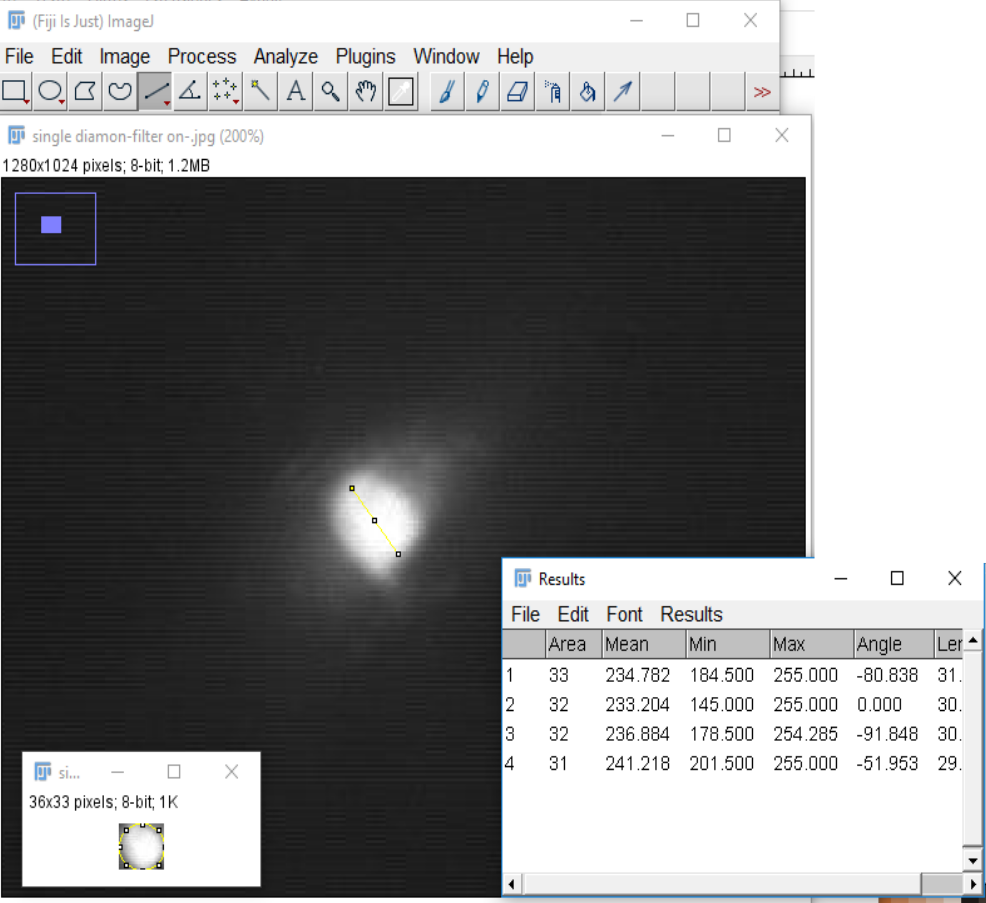
\includegraphics[width=0.7\linewidth]{../figures/Diasize4}
	\caption[Measuring of the size of the diamond]{Picture of the Software used to do the pixel measurement, in the bottom left the measurement with the overlay of circles and in the right the measurement with a direct line.}
	\label{fig:diasize4}
\end{figure}


\subsection{Fluorescence Spectrum}

As indicated in section \ref{sec:nvcentres} the NV-centres exist in a NV$^-$ and a NV$^0$ state. While the ODMR-measurements can only be done on the NV$^-$ state we need to make sure that the diamond we found has NV$^-$ centres inside.\\

Therefore the fluorescence spectrum of the diamond is recorded and the position of the ZPL is determined. In figure \ref{fig:fluorescence} we see the ZPL to be at the position $\lambda_\text{ZPL}=(645\pm3)\,\mathrm{nm}$ which corresponds to an energy of $E_\text{ZPL}=(1.922\pm0.009)\,\mathrm{eV}$. This corresponds roughly to the energy given in figure \ref{fig:nvcentres}. So we verified the existence of NV$^-$ centres in the found diamond.
\begin{figure}
	\centering
	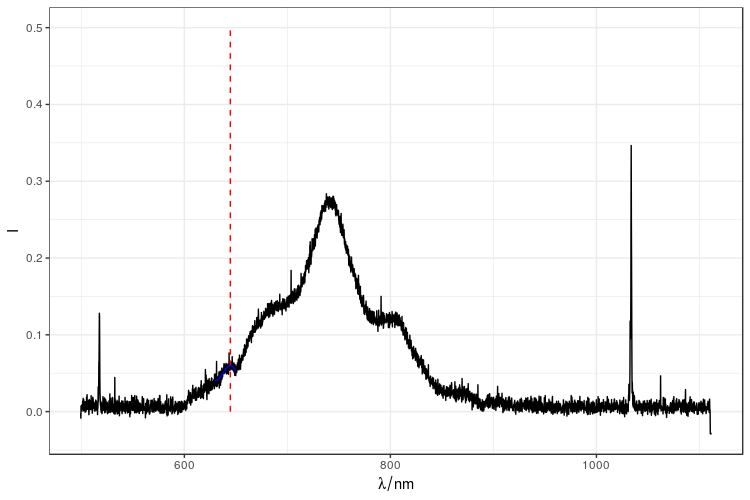
\includegraphics[width=0.8\textwidth]{../figures/fluorescence.png}
	\caption[Fluorescence spectrum of the diamond]{Fluorescence spectrum of the diamond with the zero phonon line (red line) at $\lambda_\text{ZPL}=(645\pm3)\,\mathrm{nm}$. The spectrum was achieved by averaging over 10 measurements.}
	\label{fig:fluorescence}
\end{figure}

\subsubsection{Fluorescence lifetime}

The fluorescence of the diamond was measure through the APD and the oscilloscope. A fluorescence has a relaxation time or lifetime that goes theoretically \cite{lakowicz_principles_2007}.
\begin{equation}
	I(t)=I_{0}+e^{-t/\tau}
\end{equation}
Where the intensity I decay exponentially in time and $\tau$ is the life time of the fluorescence. In the next figure the Intensity was measure in time and a fit line was add in Mathematica with the NonLinerarFit algoritm to find the lifetime.\\
\begin{figure}
	\centering
	\includegraphics[width=0.7\linewidth]{"../figures/lifetime fluorecence"}
	\caption[lifetime]{A curve fit to the intensity of the fluorescence. In blue points is the data taken from the oscilloscope and in red the fit done in Mathematica with $a+e^{-b+t}$ model}
	\label{fig:lifetime-fluorecence}
\end{figure}

\begin{array}{ccccc}
	\centering
	\text{} & \text{Estimate} & \text{Standard Error} & \text{t-Statistic} & \text{P-Value} \\
	a & 1.13398 & 0.0105947 & 107.033 & \text{3.2578056785226166$\grave{ }$*${}^{\wedge}$-301} \\
	b & -0.000165399 & 0.0119048 & -0.0140845 & \text{7.323080785918364$\grave{ }$*${}^{\wedge}$-233} \\
	\label{tab:lt}
\end{array}


As we can see in the fig \ref{fig:lifetime-fluorecence} and the table \ref{tab:lt} gives the A and B value of the  the life time is given in milliseconds $ms$.
According to this table the Fluorescence Lifetime of the NV- centres is  close to 165$ns$ that is a bit different that in literature \cite{storteboom_lifetime_2015}  but still in the same order of magnitude, that gives us a good beginning to our results.
\subsection{ODMR Measurements}

The ODMR Measurements were conducted without a magnetic field and afterwards with three magnetic fields pointing into different directions. The measured ODMR spectrum without a magnetic field is shown in figure \ref{fig:odmr-no-B}. The resonance frequency in this spectrum is determined to be $f_\text{resonance}=(2.8699\pm0.0002)\,\mathrm{GHz}$ using the calibration done in section \ref{sec:odmr-cal}.\\

In figure \ref{fig:odmr-magnet} the ODMR measurements with enabled magnetic fields are displayed. In figure \ref{fig:odmr-magnet-x} and \ref{fig:odmr-magnet-y} one can see one, respectively two resonance pairs while in \ref{fig:odmr-magnet-z} we can barely identify some peaks but cannot assign them to resonance pairs so we discarded this measurement.\\

The peaks in figure \ref{fig:odmr-magnet-x} and \ref{fig:odmr-magnet-y} we can assign to resonance pairs but the centre frequency of this resonance pairs is not equal to the measured resonance frequency of the $B=0$-measurement shown in figure \ref{fig:odmr-no-B}. So to calculate the resonance frequencies and with this the magnetic fields we used the measured frequency. Possible reasons for the shifting of this energy are discussed in section \ref{sec:summary}.

\begin{figure}
	\centering
	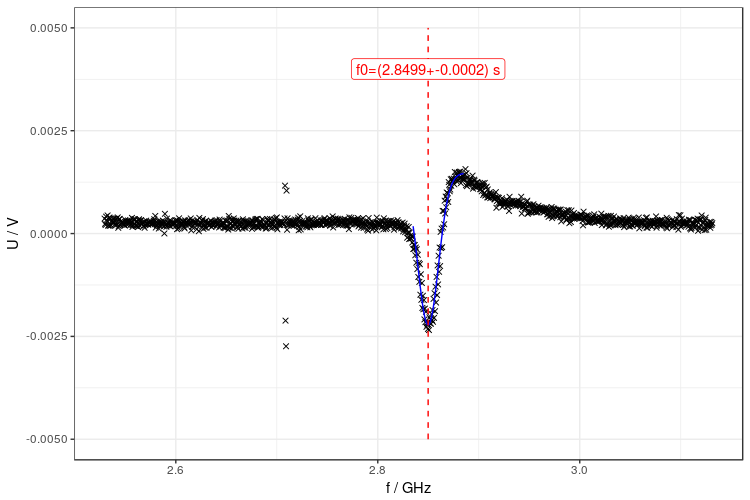
\includegraphics[width=0.8\textwidth]{../figures/odmr-1.png}
	\caption{ODMR Measurement of the diamond without a magnetic Field}
	\label{fig:odmr-no-B}
\end{figure}


\begin{figure}
	%\centering
	\begin{subfigure}{0.5\textwidth}
		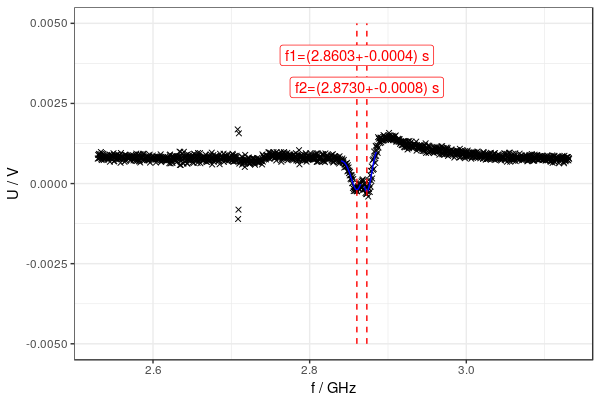
\includegraphics[width=\textwidth]{../figures/odmr-bx.png}
		\subcaption{Magnetic field in $x$-Direction}
		\label{fig:odmr-magnet-x}
	\end{subfigure}
	\begin{subfigure}{0.5\textwidth}
		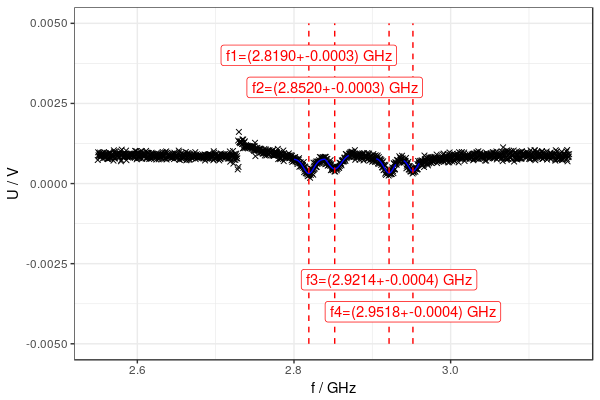
\includegraphics[width=\textwidth]{../figures/odmr-by.png}
		\subcaption{Magnetic field in $y$-Direction}
		\label{fig:odmr-magnet-y}
	\end{subfigure}
	\begin{subfigure}{0.5\textwidth}
		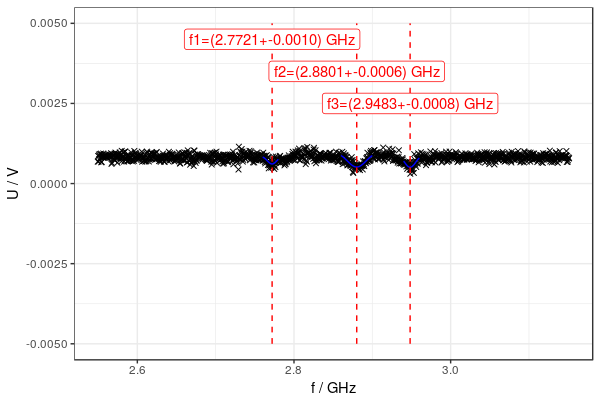
\includegraphics[width=\textwidth]{../figures/odmr-bz.png}
		\subcaption{Magnetic field in $z$-Direction}
		\label{fig:odmr-magnet-z}
	\end{subfigure}
	\caption{ODMR spectrum within a magnetic field}
	\label{fig:odmr-magnet}
\end{figure}

\begin{table}
	\centering
	\begin{tabular}{c|c|c}
		&Resonance 1&Resonance 2\\\hline
		$f_x / \mathrm{MHz}$&$6.2\pm0.5$&-\\
		$f_y / \mathrm{MHz}$&$34.7\pm0.4$&$66.5\pm0.4$\\\hline
		$B_x / \mathrm{mT}$&$0.214\pm0.018$&-\\
		$B_y / \mathrm{mT}$&$1.197\pm0.014$&$2.297\pm0.014$\\\hline
		$d_x/d$&$0.036\pm0.003$&-\\
		$d_y/d$&$0.203\pm0.002$&$0.389\pm0.002$
	\end{tabular}
	\caption{Resonance Pairs}
\end{table}